\documentclass[border=0pt]{standalone}
\usepackage{tikz}
\usetikzlibrary{calc}

\definecolor{bgtop}{HTML}{0C1F35}
\definecolor{bgbot}{HTML}{04101C}
\definecolor{steel}{HTML}{A9BCD3}
\definecolor{panel}{HTML}{2B3F66}
\definecolor{risc}{HTML}{3EE08F}
\definecolor{up}{HTML}{F5A524}
\definecolor{dir}{HTML}{38BDF8}
\definecolor{cpuc}{HTML}{C9D6E8}

% \beam{x0}{y0}{x1}{y1}{color}{opacity scale}
\newcommand{\beam}[6]{%
  \pgfmathsetmacro{\dx}{#3-#1}\pgfmathsetmacro{\dy}{#4-#2}%
  \pgfmathsetmacro{\ang}{atan2(\dy,\dx)}%
  \pgfmathsetmacro{\L}{sqrt(\dx*\dx+\dy*\dy)}%
  \pgfmathsetmacro{\w}{0.05*\L+0.08}%
  \begin{scope}[shift={(#1,#2)},rotate=\ang]
    \foreach \s/\o in {1.00/0.10, 0.65/0.18, 0.32/0.40}{
      \pgfmathsetmacro{\oo}{\o*#6}
      \fill[#5,opacity=\oo]
        (0,0) .. controls ({0.30*\L},{1.30*\w*\s}) and ({0.82*\L},{1.15*\w*\s}) .. (\L,0)
              .. controls ({0.82*\L},{-1.15*\w*\s}) and ({0.30*\L},{-1.30*\w*\s}) .. (0,0);
    }
  \end{scope}
}

% \tower{x}{ybase}{scale}
\newcommand{\tower}[3]{%
  \begin{scope}[shift={(#1,#2)},scale=#3]
    \begin{scope}[steel,line width=1.1pt,line cap=round,line join=round]
      \draw (-0.55,0) -- (-0.08,3.0);
      \draw (0.55,0) -- (0.08,3.0);
      \foreach \y/\yy in {0/0.75,0.75/1.5,1.5/2.2,2.2/3.0}{
        \pgfmathsetmacro{\xl}{-0.55+\y/3.0*0.47}\pgfmathsetmacro{\xr}{0.55-\y/3.0*0.47}
        \pgfmathsetmacro{\xll}{-0.55+\yy/3.0*0.47}\pgfmathsetmacro{\xrr}{0.55-\yy/3.0*0.47}
        \draw[line width=0.7pt] (\xl,\y) -- (\xrr,\yy);
        \draw[line width=0.7pt] (\xr,\y) -- (\xll,\yy);
        \draw[line width=0.7pt] (\xll,\yy) -- (\xrr,\yy);
      }
    \end{scope}
    \fill[panel,rounded corners=2pt,draw=steel,line width=1pt] (-0.30,2.95) rectangle (0.30,4.15);
    \foreach \i in {0,1}{\foreach \j in {0,...,4}{
      \fill[white,opacity=0.9] ({-0.14+\i*0.28},{3.12+\j*0.22}) circle (0.045);
    }}
  \end{scope}
}

% \ris{x}{y}: reconfigurable intelligent surface (tilted panel of elements)
\newcommand{\ris}[2]{%
  \begin{scope}[shift={(#1,#2)}]
    \fill[risc,opacity=0.10] (0,0) circle (1.25);
    \fill[risc,opacity=0.12] (0,0) circle (0.85);
    \fill[risc!20!black,rounded corners=2pt,draw=risc,line width=1.2pt] (-0.55,-0.75) rectangle (0.55,0.75);
    \foreach \i in {0,...,3}{\foreach \j in {0,...,4}{
      \fill[risc,opacity=0.85] ({-0.43+\i*0.26},{-0.62+\j*0.26}) rectangle ++(0.16,0.16);
    }}
  \end{scope}
}

% \phone{x}{y}
\newcommand{\phone}[2]{%
  \begin{scope}[shift={(#1,#2)}]
    \fill[up,opacity=0.18] (0,0) circle (0.70);
    \fill[up,opacity=0.22] (0,0) circle (0.47);
    \fill[black!85,rounded corners=2.4pt] (-0.22,-0.40) rectangle (0.22,0.40);
    \draw[up,line width=1.1pt,rounded corners=2.4pt] (-0.22,-0.40) rectangle (0.22,0.40);
    \fill[up!30!black,rounded corners=1pt] (-0.17,-0.30) rectangle (0.17,0.31);
    \fill[black!85] (-0.055,0.32) rectangle (0.055,0.36);
    \draw[up,line width=0.9pt,-latex] (0,-0.18) -- (0,0.17);
  \end{scope}
}

\begin{document}
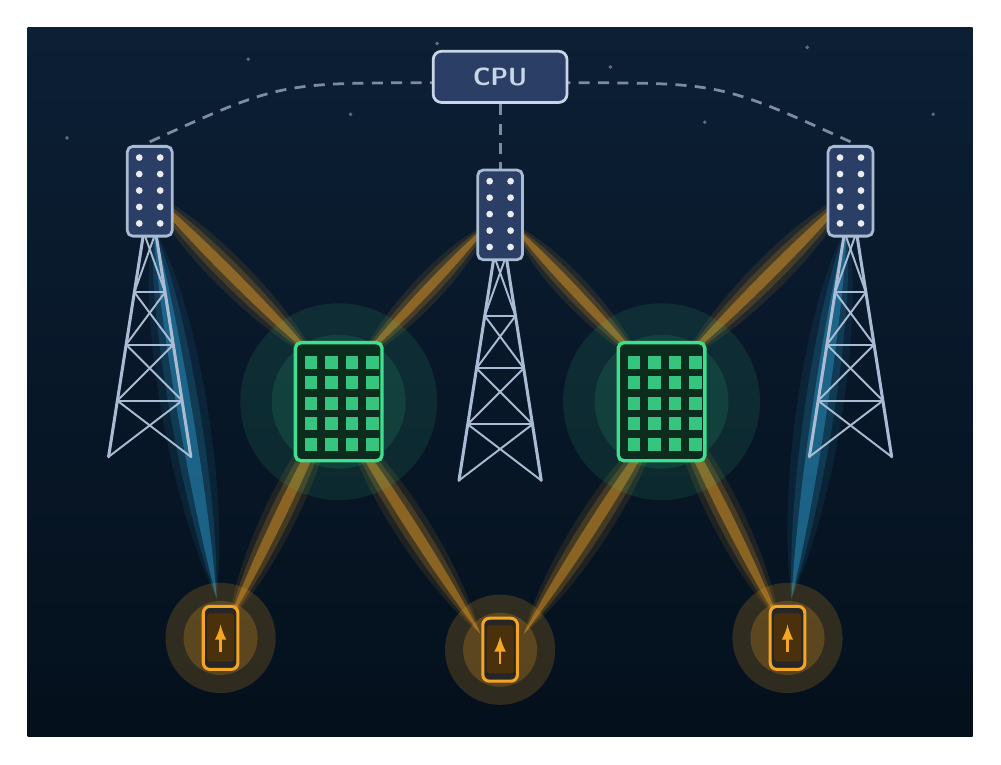
\begin{tikzpicture}
  \useasboundingbox (0,0) rectangle (12,9);
  \clip (0,0) rectangle (12,9);
  \shade[top color=bgtop,bottom color=bgbot] (0,0) rectangle (12,9);
  \foreach \x/\y in {2.8/8.6,5.2/8.8,7.4/8.5,9.9/8.75,11.5/7.9,0.5/7.6,4.1/7.9,8.6/7.8}{
    \fill[white,opacity=0.35] (\x,\y) circle (0.025);
  }

  % CPU and fronthaul
  \fill[panel,rounded corners=3pt,draw=cpuc,line width=1pt] (5.15,8.05) rectangle (6.85,8.70);
  \node[text=cpuc,font=\sffamily\bfseries\small] at (6.00,8.375) {CPU};
  \draw[cpuc,opacity=0.6,line width=1pt,dash pattern=on 4pt off 3pt] (1.55,7.55) .. controls (3.2,8.3) .. (5.15,8.30);
  \draw[cpuc,opacity=0.6,line width=1pt,dash pattern=on 4pt off 3pt] (10.45,7.55) .. controls (8.8,8.3) .. (6.85,8.30);
  \draw[cpuc,opacity=0.6,line width=1pt,dash pattern=on 4pt off 3pt] (6.00,7.15) -- (6.00,8.05);

  % uplink beams: UE -> RIS -> BS (amber) and direct UE -> BS (blue)
  \beam{2.55}{1.45}{3.85}{4.15}{up}{1}
  \beam{5.75}{1.30}{4.05}{3.95}{up}{1}
  \beam{6.30}{1.30}{8.00}{3.95}{up}{1}
  \beam{9.55}{1.45}{8.20}{4.15}{up}{1}
  \beam{3.70}{4.75}{1.55}{6.90}{up}{1}
  \beam{4.20}{4.75}{5.85}{6.50}{up}{1}
  \beam{7.80}{4.75}{6.15}{6.50}{up}{1}
  \beam{8.30}{4.75}{10.45}{6.90}{up}{1}
  \beam{2.40}{1.75}{1.60}{6.45}{dir}{0.8}
  \beam{9.70}{1.75}{10.40}{6.45}{dir}{0.8}

  % RISs, BS towers, users
  \ris{3.95}{4.25}
  \ris{8.05}{4.25}
  \tower{1.55}{3.55}{0.95}
  \tower{6.00}{3.25}{0.95}
  \tower{10.45}{3.55}{0.95}
  \phone{2.45}{1.25}
  \phone{6.00}{1.10}
  \phone{9.65}{1.25}
\end{tikzpicture}
\end{document}
